% file: triangulation-select-k.tex

\documentclass[tikz]{standalone}

\usetikzlibrary{positioning, chains}

\begin{document}
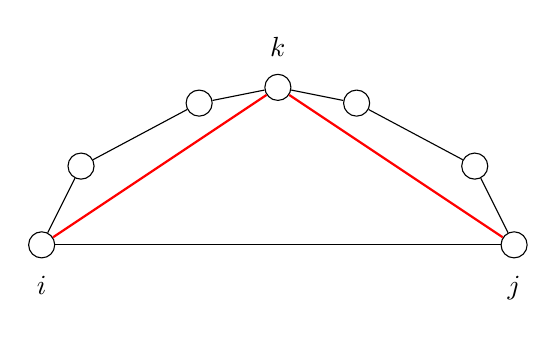
\begin{tikzpicture}[node distance = 0.10cm]
  \foreach \p/\n in {{0,0}/1, {0.5,1}/2, {2,1.8}/3, {3,2}/4, {4, 1.8}/5, {5.5,1}/6, {6,0}/7} {
    \node (\n) [draw, circle, minimum size = 6pt] at (\p) {};
  }

  \path (1) edge (2)
  	(2) edge (3)
	(3) edge (4)
	(4) edge (5)
	(5) edge (6)
	(6) edge (7)
	(7) edge (1);

  \node (i) [below = of 1] {$i$};
  \node (j) [below = of 7] {$j$};
  \node (k) [above = of 4] {$k$};

  \draw[red, thick] (1) to (4);
  \draw[red, thick] (4) to (7);
\end{tikzpicture}
\end{document}
